\section{Deliverables}

\epigraph{\emph{Dr.\ Long, put down the Rilke and step away from the
computer.}}{---Michael Olson}

You will need to turn in the following source code and header files:

\begin{enumerate}
  \item Your program \emph{must} have the following source and header
    files:
  \begin{itemize}
    \item \texttt{batcher.c} implements Batcher Sort.
    \item \texttt{batcher.h} specifies the interface to \texttt{batcher.c}.
    \item \texttt{insert.c} implements Insertion Sort.
    \item \texttt{insert.h} specifies the interface to \texttt{insert.c}.
    \item \texttt{heap.c} implements Heap Sort.
    \item \texttt{heap.h} specifies the interface to \texttt{heap.c}.
    \item \texttt{quick.c} implements recursive Quicksort.
    \item \texttt{quick.h} specifies the interface to \texttt{quick.c}.
    \item \texttt{set.h} implements and specifies the interface for the
      set ADT.
    \item \texttt{stats.c} implements the statistics module.
    \item \texttt{stats.h} specifies the interface to the statistics
      module.
    \item \texttt{sorting.c} contains \texttt{main()} and \emph{may}
      contain any other functions necessary to complete the assignment.
  \end{itemize}
\end{enumerate}

You can have other source and header files, but \emph{do not try to be
overly clever}. \textcolor{red}{The header files for each of the sorts
are provided to you and may not be modified.} Each sort function takes a
pointer to a \texttt{Stats} \texttt{struct}, the array of
\texttt{uint32\_t}s to sort as the first parameter, and the length of
the array as the second parameter. You will also need to turn in the
following:

\begin{enumerate}
  \item \texttt{Makefile}:
    \begin{itemize}
      \item \texttt{CC = clang} must be specified.
      \item \texttt{CFLAGS = -Wall -Wextra -Werror -Wpedantic} must be specified.
      \item \texttt{make} must build the \texttt{sorting}
        executable, as should \texttt{make all} and \texttt{make
        sorting}.
      \item \texttt{make clean} must remove all files that are compiler
        generated.
      \item \texttt{make format} should format all your source code,
        including the header files.
    \end{itemize}
  \item \texttt{README.md}: This must use proper Markdown syntax. It
    must describe how to use your program and \texttt{Makefile}. It
    should also list and explain any command-line options that your
    program accepts. Any false positives reported by \texttt{scan-build}
    should be documented and explained here as well. Note down any known
    bugs or errors in this file as well for the graders.
  \item \texttt{DESIGN.pdf}: This document \emph{must} be a proper
    PDF\@. This design document must describe your design and design
    process for your program with enough detail such that a sufficiently
    knowledgeable programmer would be able to replicate your
    implementation. \textcolor{red}{This does not mean copying your
    entire program in verbatim}. You should instead describe how your
    program works with supporting pseudocode.
  \item \texttt{WRITEUP.pdf}: This document \emph{must} be a PDF. The
    writeup must include the following:
    \begin{itemize}
      \item What you learned from the different sorting algorithms.
        Under what conditions do sorts perform well? Under what
        conditions do sorts perform poorly? What conclusions can you
        make from your findings?
      \item Graphs explaining the performance of the sorts on a variety
        of inputs, such as arrays in reverse order, arrays with a small
        number of elements, and arrays with a large number of elements. Your
        graphs must be produced using either \texttt{gnuplot} or
        \texttt{matplotlib}. You will find it helpful to write a script to
        handle the plotting. As always, \texttt{awk} will be helpful for parsing
        the output of your program.
      \item Analysis of the graphs you produce. Here is an example graph
        produced by \texttt{gnuplot} with a different set of sorts for reference
        (axes are log-scaled):
        \begin{center}
          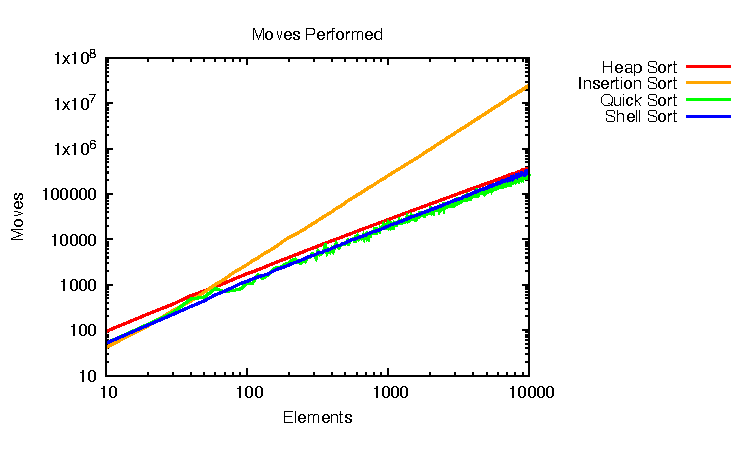
\includegraphics[width=0.8\textwidth]{images/moves.pdf} \\
        \end{center}
        You should look carefully at any graphs that you produce. Are
        all of the lines smooth? For example, in this graph there are
        some features of interest. What could be causing features that
        appear in your own graphs?
    \end{itemize}
\end{enumerate}
